\problemname{Lasta färjan}
En bilfärja ska lastas med bilar, och en samling bilar står på kö för att komma med färjan. Tiden mellan turerna är väldigt lång, och därför är det viktigt för de resande att så många bilar som möjligt kan komma med färjan vid en sådan tur. Bolaget Kass Sjöfart AB (som driver bilfärjan) har på sistone mottagit ett stort antal klagobrev från en organisation som kallar sig \emph{Arga Unga Algoritmiker} som menar att packningen av bilar på färjan är \emph{``dålig''}, \emph{``suboptimal''}, \emph{``heuristisk''} och \emph{``ohållbar''}. Bolagets verkställande direktör Ernst E. Kass bekräftar att man slarvat vid packningen av färjan, och går nu ut med ett uttalande om att man hädanefter alltid kommer att packa färjan så att så många bilar som möjligt kommer med. Hur man ska lyckas med det har Ernst inte velat svara på, men ryktet säger att man bett den svenska Programmeringsolympiaden om hjälp.

Bilfärjan har fyra filer, där varje fil har en viss längd i meter, och alla filar är lika långa. En samling bilar står på kö för att få åka ombord på färjan, och bilarna kommer att åka på färjan i den ordning som de står i kön. Personalen på färjan kan dock välja vilken fil som en viss bil ska åka in i (givet att den får plats). När en bil inte längre får plats i någon av filerna så anses färjan vara fullastad (man hoppar alltså inte över bilar). Dessutom är det viktigt att det är minst en meters avstånd mellan varje par av bilar som står intill varandra i samma fil (ifall det skulle börja gunga, och bilarna sätts i rörelse).

Du kommer att få veta hur lång färjan är, och vilka bilar som står i kön. Din uppgift är att hjälpa färjepersonalen med att räkna ut hur många bilar man som mest kan lasta, om man är smart när man väljer fil åt bilarna.

\begin{figure}[!h]
\begin{center}
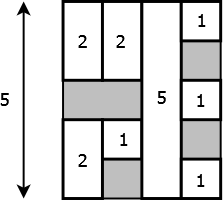
\includegraphics[scale=0.5]{farjan}
\end{center}
\caption{Ett exempel på hur färjan kan se ut efter en optimal packning. Färjan är $5$ meter lång, och längden på bilarna som stod i kön är $2, 1, 2, 5, 1, 1, 2, 1, 1, 2$, varav bara de första $8$ fick plats på färjan.}
\label{fig1}
\end{figure}

\section*{Indata}
På första raden i indata står ett heltal $N$, antal bilar. Antalet bilar i kön är max $200$. På andra raden i indata står ett heltal $L$, längden på filerna. Filerna är inte längre än $60$ meter. Sedan följer $N$ heltal på en rad (separerade av mellanslag), där varje heltal beskriver längden på en bil. Bilarna är minst $1$ meter långa och högst $10$ meter långa och samtidigt högst L. Bilarna först i denna sekvens är de som står först i kön.

\section*{Utdata}
Utdata ska bestå av ett enda heltal: det högsta antal bilar som får plats på färjan.

\section*{Poängsättning}
Din lösning kommer att testas på en mängd testfallsgrupper.
För att få poäng för en grupp så måste du klara alla testfall i gruppen.

\noindent
\begin{tabular}{| l | l | p{12cm} |}
  \hline
  \textbf{Grupp} & \textbf{Poäng} & \textbf{Gränser} \\ \hline
  $1$    & $40$        & $N \le 20, L \le 40$ \\ \hline 
  $2$    & $60$        & Inga ytterligare begränsningar. \\ \hline 
\end{tabular}
